% ===================================================================
%  Week 15 — Sequence Recognition & OCR for DocScan
%  Session 2 of 2: CRNN + CTC --- training, decoding, and evaluation
% ===================================================================
\documentclass[10pt,aspectratio=169]{beamer}
% ===================================================================
%  Shared Beamer preamble for "Practical Image Processing"
%  English slides. Compile with pdfLaTeX.
% ===================================================================

\usetheme{metropolis}
\usepackage[T1]{fontenc}
\usepackage[utf8]{inputenc}
\usepackage{lmodern}
\usepackage{listings}
\usepackage{tcolorbox}
\usepackage{fontawesome5}
\usepackage{booktabs}
\usepackage{amsmath,amssymb}
\usepackage{tikz}
\usepackage{pgfplots}
\pgfplotsset{compat=1.17}
\usetikzlibrary{arrows.meta,positioning,shapes.geometric,fit,backgrounds,matrix}
\tcbuselibrary{skins,breakable}

% ---- Palette --------------------------------------------------------
\definecolor{coursePrimary}{HTML}{1B4965}   % deep blue
\definecolor{courseAccent}{HTML}{E76F51}    % coral
\definecolor{courseGood}{HTML}{2A9D8F}      % teal
\definecolor{courseBad}{HTML}{C0392B}       % red
\definecolor{courseInfo}{HTML}{2980B9}      % blue
\definecolor{codeBg}{HTML}{F5F6FA}
\definecolor{codeKw}{HTML}{8E44AD}
\definecolor{codeStr}{HTML}{2A9D8F}
\definecolor{codeCom}{HTML}{7F8C8D}

\setbeamercolor{frametitle}{bg=coursePrimary}
\setbeamercolor{progress bar}{fg=courseAccent}
\setbeamercolor{alerted text}{fg=courseAccent}
\metroset{block=fill,sectionpage=progressbar,numbering=fraction}

% ---- Code listings (Python is built into listings) -----------------
\lstdefinestyle{course}{
  backgroundcolor=\color{codeBg},
  basicstyle=\ttfamily\scriptsize,
  keywordstyle=\color{codeKw}\bfseries,
  stringstyle=\color{codeStr},
  commentstyle=\color{codeCom}\itshape,
  numberstyle=\tiny\color{codeCom},
  numbers=left, numbersep=6pt,
  showstringspaces=false, breaklines=true, breakatwhitespace=true,
  tabsize=4, columns=fullflexible,
  frame=single, framesep=4pt, rulecolor=\color{gray!30},
  keepspaces=true, upquote=true, language=Python,
}
\lstset{style=course}
\lstdefinelanguage{bash}{
  keywords={cd,pip,python,venv,source,import}, sensitive=true,
  morecomment=[l]{\#}, morestring=[b]', morestring=[b]",
}

% ---- Reusable callout boxes ----------------------------------------
\newtcolorbox{goodbox}[1][Good practice]{colback=courseGood!8,colframe=courseGood,
  fonttitle=\bfseries,title={\faCheck~#1},boxrule=0.6pt,left=4pt,right=4pt,top=3pt,bottom=3pt}
\newtcolorbox{badbox}[1][Pitfall]{colback=courseBad!8,colframe=courseBad,
  fonttitle=\bfseries,title={\faTimes~#1},boxrule=0.6pt,left=4pt,right=4pt,top=3pt,bottom=3pt}
\newtcolorbox{infobox}[1][Note]{colback=courseInfo!8,colframe=courseInfo,
  fonttitle=\bfseries,title={\faInfoCircle~#1},boxrule=0.6pt,left=4pt,right=4pt,top=3pt,bottom=3pt}
\newtcolorbox{mathbox}[1][Math]{colback=coursePrimary!6,colframe=coursePrimary,
  fonttitle=\bfseries,title={\faCalculator~#1},boxrule=0.6pt,left=4pt,right=4pt,top=3pt,bottom=3pt}

\newcommand{\keyidea}[1]{\begin{alertblock}{Key idea}#1\end{alertblock}}
\newcommand{\term}[1]{\textbf{\color{coursePrimary}#1}}
\newcommand{\code}[1]{\lstinline[basicstyle=\ttfamily\small]|#1|}

% ---- A helper to draw a small pixel grid, cells shaded by value ----
% \pixelgrid{ {10,20,120,200,240}, {30,60,130,180,230}, ... }
\newcommand{\pixelgrid}[1]{%
  \begin{tikzpicture}[font=\scriptsize,scale=0.6]
    \foreach \row [count=\ry] in {#1} {
      \foreach \val [count=\cx] in \row {
        \draw[gray,fill=coursePrimary!8] (\cx,-\ry) rectangle ++(1,-1);
        \node at (\cx+0.5,-\ry-0.5) {\val};
      }
    }
  \end{tikzpicture}}


\title{Sequence Recognition \& OCR}
\subtitle{Week 15 — Session 2: CRNN, CTC, decoding, and edit distance}
\author{Practical Image Processing}
\date{Lecture 15.2 \textbullet\ 60--70 min}

\begin{document}

\maketitle

\begin{frame}{Recap of Session 1}
  \begin{columns}[T]
    \begin{column}{0.58\textwidth}
      \begin{itemize}
        \item Segment-then-classify multiplies errors: a 97\% digit reader is only $\sim$83\% at 6 digits.
        \item Cutting fails on touching digits and odometer roll-over.
        \item End-to-end fix: CNN $\rightarrow$ a sequence of \term{feature columns} $\rightarrow$ RNN $\rightarrow$ per-column scores.
        \item Left open: the \emph{alignment problem} --- $T$ columns vs.\ $L$ characters, with the collapse rule as a hint.
      \end{itemize}
    \end{column}
    \begin{column}{0.42\textwidth}
      \begin{alertblock}{Today's job}
        Make the CRNN concrete, meet \term{CTC} that trains it without cut marks, decode its output,
        and evaluate honestly with edit distance --- then ship the reader.
      \end{alertblock}
    \end{column}
  \end{columns}
\end{frame}

\begin{frame}{Roadmap --- Session 2}\tableofcontents\end{frame}

% ==================================================================
\section{The CRNN in detail}
% ==================================================================

\begin{frame}{The three stages of a CRNN}
  \begin{center}
  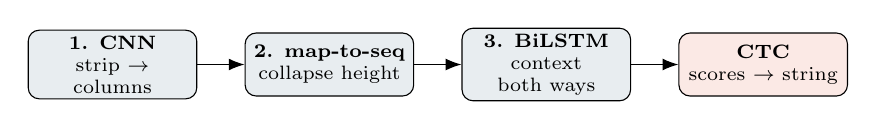
\begin{tikzpicture}[font=\scriptsize,node distance=4mm and 6mm,
      box/.style={draw,rounded corners,fill=coursePrimary!10,minimum height=8mm,inner sep=2pt,text width=20mm,align=center}]
    \node[box] (cnn) {\textbf{1. CNN}\\ strip $\to$ columns};
    \node[box,right=of cnn] (m2s) {\textbf{2. map-to-seq}\\ collapse height};
    \node[box,right=of m2s] (rnn) {\textbf{3. BiLSTM}\\ context both ways};
    \node[box,right=of rnn,fill=courseAccent!15] (ctc) {\textbf{CTC}\\ scores $\to$ string};
    \draw[-{Latex[length=2mm]}] (cnn)--(m2s);
    \draw[-{Latex[length=2mm]}] (m2s)--(rnn);
    \draw[-{Latex[length=2mm]}] (rnn)--(ctc);
  \end{tikzpicture}
  \end{center}
  \begin{itemize}
    \item \textbf{Convolutional} layers extract features while keeping the width axis.
    \item \textbf{Recurrent} layers read those columns left-to-right \emph{and} right-to-left.
    \item The \textbf{transcription} layer (CTC) turns per-column scores into the final reading.
  \end{itemize}
\end{frame}

\begin{frame}{Stage 1: CNN, tracking the shape}
  \begin{center}
  \begin{tabular}{@{}lll@{}}
    \toprule
    \textbf{Stage} & \textbf{Output} $(C\times H\times W)$ & \textbf{Note} \\
    \midrule
    Input strip           & $1\times 8\times 48$   & 6 digits, $8{\times}8$ each \\
    Conv1 + pool $2{\times}2$ & $16\times 4\times 24$ & shrink both axes \\
    Conv2 + pool $2{\times}2$ & $32\times 2\times 12$ & depth grows \\
    Conv3 + pool $2{\times}1$ & $32\times 1\times 12$ & \alert{height $\to$ 1, width kept} \\
    Squeeze height        & $32\times 12$          & a length-12 sequence \\
    \bottomrule
  \end{tabular}
  \end{center}
  \begin{itemize}
    \item The final pool is $2\times1$: it removes the last of the height but leaves width alone.
    \item Result: $T{=}12$ columns, each a 32-d feature vector --- the sequence the RNN reads.
  \end{itemize}
\end{frame}

\begin{frame}{Stage 2: map-to-sequence}
  \begin{itemize}
    \item The CNN tensor is $C\times 1\times T$. Squeeze the height, then \term{permute} to $T\times C$.
    \item Now the data is literally a sequence: ``time'' $=$ horizontal position, ``features'' $=$ channels.
    \item Column $t$ carries what the CNN saw in a vertical slice around image-x $\approx 4t$ (its receptive field).
  \end{itemize}
  \begin{mathbox}
    tensor $(C,1,T) \;\to\; \text{squeeze} \;\to\; (C,T) \;\to\; \text{permute} \;\to\; (T,C)$
  \end{mathbox}
\end{frame}

\begin{frame}{Stage 3: BiLSTM adds context}
  \begin{itemize}
    \item Each column enters an \term{LSTM}, a recurrent unit that carries a memory along the sequence.
    \item \term{Bidirectional}: one pass left$\to$right, one right$\to$left; concatenate. Every column now
          knows what came before \emph{and} after it.
    \item A linear layer maps each column's hidden state to \term{class scores}: 10 digits $+$ 1 blank $= 11$.
  \end{itemize}
  \begin{goodbox}
    This is why a half-rolled digit can still be read: its neighbours constrain what it must be.
  \end{goodbox}
\end{frame}

\begin{frame}{The output we now have}
  \begin{center}
  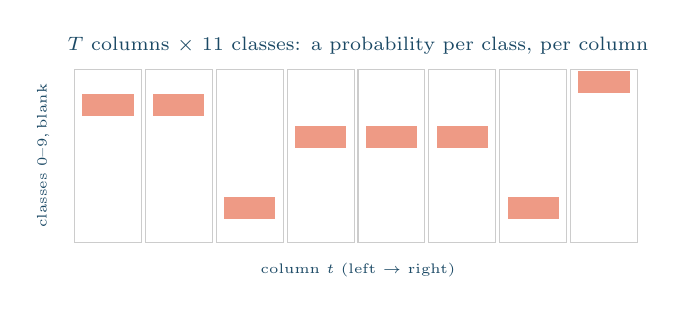
\begin{tikzpicture}[font=\scriptsize]
    % a T x classes grid, sketch probabilities
    \foreach \t in {0,...,7} {
      \draw[gray!40] (\t*0.9,0) rectangle ++(0.85,2.2);
    }
    \node[coursePrimary] at (3.6,2.5) {$T$ columns $\times$ 11 classes: a probability per class, per column};
    \node[coursePrimary,rotate=90,font=\tiny] at (-0.4,1.1) {classes 0--9,\,blank};
    \node[coursePrimary,font=\tiny] at (3.6,-0.35) {column $t$ (left $\to$ right)};
    % highlight argmax path
    \foreach \t/\h in {0/1.6,1/1.6,2/0.3,3/1.2,4/1.2,5/1.2,6/0.3,7/1.9} {
      \fill[courseAccent!70] (\t*0.9+0.1,\h) rectangle ++(0.65,0.28);
    }
  \end{tikzpicture}
  \end{center}
  \begin{itemize}
    \item For every column we have a full probability distribution over the 11 classes.
    \item Coral cells = the most probable class per column (the ``best path'').
    \item But how do we \emph{train} this, and turn it into one string? Enter CTC.
  \end{itemize}
\end{frame}

% ==================================================================
\section{CTC: training without alignment}
% ==================================================================

\begin{frame}{The blank symbol, precisely}
  \begin{itemize}
    \item Add one extra class, the \term{blank} \code{-}: ``emit no new character at this column.''
    \item A raw per-column output (a \term{path}) is collapsed to text by two rules, \emph{in order}:
    \begin{enumerate}
      \item merge \emph{adjacent equal} labels into one, then
      \item delete all blanks.
    \end{enumerate}
    \item The blank is what lets a genuine \emph{double} letter survive.
  \end{itemize}
  \begin{mathbox}[Two paths, same length, different meaning]
    \code{7\,7\,7} $\to$ \code{7} \qquad but \qquad \code{7\,-\,7} $\to$ \code{77}
  \end{mathbox}
\end{frame}

\begin{frame}{Many paths spell the same string}
  Target \code{42}, with $T{=}4$ columns and alphabet $\{4,2,-\}$. All of these collapse to \code{42}:
  \begin{center}
  \begin{tabular}{@{}ll@{\hspace{2em}}ll@{}}
    \toprule
    path & collapses to & path & collapses to \\
    \midrule
    \code{4\,4\,2\,2} & \code{42} & \code{-\,4\,2\,-} & \code{42} \\
    \code{4\,2\,2\,2} & \code{42} & \code{4\,-\,2\,2} & \code{42} \\
    \code{4\,4\,4\,2} & \code{42} & \code{4\,2\,-\,-} & \code{42} \\
    \bottomrule
  \end{tabular}
  \end{center}
  \begin{itemize}
    \item Many distinct column-paths correspond to the \emph{one} reading we want.
    \item We never chose which path is ``right'' --- and we don't have to.
  \end{itemize}
\end{frame}

\begin{frame}{The CTC idea: sum over all alignments}
  \begin{itemize}
    \item Probability of a \emph{path} = product of its per-column probabilities (columns treated as independent given the features).
    \item Probability of the \emph{label} = \alert{sum} of the probabilities of \emph{all} paths that collapse to it.
    \item \term{CTC loss} = $-\log$ of that summed probability. Training pushes it up --- for \emph{every} valid alignment at once.
  \end{itemize}
  \begin{mathbox}[Connectionist Temporal Classification]
    $\displaystyle P(\ell \mid x) = \sum_{\pi\,:\,\mathcal{B}(\pi)=\ell} \prod_{t=1}^{T} p_t(\pi_t)$,
    \qquad $\text{loss}=-\log P(\ell\mid x)$
  \end{mathbox}
  \keyidea{No cut marks needed: CTC lets the network discover the alignment by rewarding \emph{all} of them.}
\end{frame}

\begin{frame}{CTC by hand, tiny example}
  Alphabet $\{a,-\}$, $T{=}2$, target \code{a}. Say per-column probabilities are:
  \begin{center}
  \begin{tabular}{@{}lcc@{}}
    \toprule
     & $p(a)$ & $p(-)$ \\
    \midrule
    column 1 & 0.7 & 0.3 \\
    column 2 & 0.6 & 0.4 \\
    \bottomrule
  \end{tabular}
  \end{center}
  Paths collapsing to \code{a}: \code{a\,a}, \code{a\,-}, \code{-\,a}.
  \begin{mathbox}
    $P(\text{\code{a}}) = \underbrace{0.7{\cdot}0.6}_{aa}+\underbrace{0.7{\cdot}0.4}_{a-}+\underbrace{0.3{\cdot}0.6}_{-a}
    = 0.42+0.28+0.18 = 0.88$
  \end{mathbox}
  Loss $= -\log 0.88 \approx 0.128$. The only excluded path is \code{-\,-} (collapses to empty).
\end{frame}

\begin{frame}{Why summing is tractable}
  \begin{itemize}
    \item The number of paths is exponential in $T$ --- we cannot enumerate them for real strips.
    \item But the collapse rule has structure: a \term{dynamic-programming} pass (the ``forward algorithm'')
          sums all alignments in $O(T\cdot L)$ time.
    \item You never implement this yourself --- \code{nn.CTCLoss} does it, differentiably.
  \end{itemize}
  \begin{goodbox}
    Same trick as summing paths through a lattice: reuse partial sums instead of re-walking every route.
  \end{goodbox}
\end{frame}

% ==================================================================
\section{Decoding \& evaluation}
% ==================================================================

\begin{frame}{Greedy (best-path) decoding}
  \begin{itemize}
    \item At \emph{inference} we want one string. Simplest: take the \code{argmax} class in each column\ldots
    \item \ldots then apply the collapse rule (merge repeats, drop blanks). This is \term{greedy decoding}.
    \item Fast and usually good, but it commits column-by-column and can miss the truly best \emph{string}.
  \end{itemize}
  \begin{mathbox}[Greedy on our example]
    argmax per column: \code{4\,4\,-\,2\,2\,-\,6\,6} $\to$ merge $\to$ \code{4\,-\,2\,-\,6}
    $\to$ drop blanks $\to$ \code{426}
  \end{mathbox}
\end{frame}

\begin{frame}{Beam search decoding}
  \begin{itemize}
    \item Greedy can be wrong: the best \emph{path} is not always the best \emph{string} (many paths vote for a string).
    \item \term{Beam search} keeps the top-$k$ partial strings, accumulating the summed probability per string.
    \item More faithful to the CTC objective; costs more compute. A language model can be folded in here.
  \end{itemize}
  \begin{goodbox}[Rule of thumb]
    Start with greedy; reach for beam search only if the greedy reading is not accurate enough.
  \end{goodbox}
\end{frame}

\begin{frame}{Evaluating a reader: not just ``right/wrong''}
  \begin{itemize}
    \item \term{Sequence accuracy}: fraction of readings that are \emph{exactly} correct. Strict --- one wrong digit fails the whole string.
    \item \term{Character error rate (CER)}: how many single-character edits to fix the reading, per character.
    \item CER is the humane metric: it credits a reading that is off by one digit instead of scoring it zero.
  \end{itemize}
  \keyidea{Report both: sequence accuracy for ``did we nail it,'' CER for ``how close were we.''}
\end{frame}

\begin{frame}{Edit distance (Levenshtein)}
  \begin{itemize}
    \item The \term{edit distance} between two strings = fewest single-character \emph{insertions, deletions, substitutions} to turn one into the other.
    \item Computed by a small dynamic-programming table --- the same lattice idea as CTC's forward pass.
  \end{itemize}
  \begin{mathbox}[The recurrence]
    $\displaystyle D[i,j]=\min\begin{cases} D[i{-}1,j]+1 & \text{(delete)}\\ D[i,j{-}1]+1 & \text{(insert)}\\ D[i{-}1,j{-}1]+\mathbb{1}[a_i\neq b_j] & \text{(match/sub)}\end{cases}$
  \end{mathbox}
\end{frame}

\begin{frame}{Edit distance, worked}
  Reference \code{018426}, prediction \code{018326}. Walk the strings:
  \begin{center}
  \begin{tabular}{@{}ccccccc@{}}
    \toprule
    pos & 1 & 2 & 3 & 4 & 5 & 6 \\
    \midrule
    ref  & 0 & 1 & 8 & \alert{4} & 2 & 6 \\
    pred & 0 & 1 & 8 & \alert{3} & 2 & 6 \\
    \bottomrule
  \end{tabular}
  \end{center}
  \begin{itemize}
    \item One substitution ($4\!\to\!3$): edit distance $=1$.
    \item CER $= 1/6 \approx 0.167$; sequence accuracy for this reading $=0$ (not exactly correct).
    \item A pipeline that never gets the whole string but is usually off by one still has a \emph{low CER}.
  \end{itemize}
\end{frame}

\begin{frame}{Insertions and deletions matter too}
  \begin{itemize}
    \item If the reader drops a digit (\code{01826} for \code{018426}) that is a \term{deletion}, distance $1$.
    \item If it hallucinates one (\code{0184426}) that is an \term{insertion}, distance $1$.
    \item Length changes are exactly why we need edit distance, not a position-by-position compare.
  \end{itemize}
  \begin{badbox}
    Comparing character-by-character at fixed positions breaks the moment the reading is one digit too short
    or too long --- everything after the slip looks wrong. Edit distance handles it correctly.
  \end{badbox}
\end{frame}

% ==================================================================
\section{Code walkthrough}
% ==================================================================

\begin{frame}[fragile]{The CRNN in PyTorch}
\begin{lstlisting}[language=Python]
class CRNN(nn.Module):
    def __init__(self, n_classes=11):   # 10 digits + blank
        super().__init__()
        self.cnn = nn.Sequential(
            nn.Conv2d(1, 16, 3, padding=1), nn.ReLU(), nn.MaxPool2d(2),
            nn.Conv2d(16, 32, 3, padding=1), nn.ReLU(), nn.MaxPool2d(2),
            nn.Conv2d(32, 32, 3, padding=1), nn.ReLU(),
            nn.MaxPool2d((2, 1)))                 # height->1, width kept
        self.rnn = nn.LSTM(32, 64, bidirectional=True, batch_first=False)
        self.fc  = nn.Linear(128, n_classes)      # 64*2 -> classes
    def forward(self, x):                         # x: (B,1,8,W)
        f = self.cnn(x)                           # (B,32,1,T)
        f = f.squeeze(2).permute(2, 0, 1)         # (T,B,32)
        y, _ = self.rnn(f)                        # (T,B,128)
        return self.fc(y).log_softmax(2)          # (T,B,n_classes)
\end{lstlisting}
  The three CRNN stages, line for line: \code{cnn}, then map-to-sequence, then \code{rnn}+\code{fc}.
\end{frame}

\begin{frame}[fragile]{Training with CTCLoss}
\begin{lstlisting}[language=Python]
ctc = nn.CTCLoss(blank=10, zero_infinity=True)
for xb, targets, in_lens, tgt_lens in loader:
    opt.zero_grad()
    logp = net(xb)                    # (T, B, 11) log-probs
    loss = ctc(logp, targets, in_lens, tgt_lens)
    loss.backward(); opt.step()
\end{lstlisting}
  \begin{itemize}
    \item \code{logp}: log-probabilities, shape (time, batch, classes) --- CTC's required layout.
    \item \code{in\_lens}: how many columns each sample really has ($T$); \code{tgt\_lens}: each label's length ($L$).
    \item \code{blank=10}: the blank is class index 10. One call sums over \emph{all} alignments for you.
  \end{itemize}
  \begin{badbox}
    Getting \code{blank} index or the (T,B,C) order wrong is the \#1 CTC bug --- loss goes to \code{inf} or \code{nan}.
  \end{badbox}
\end{frame}

\begin{frame}[fragile]{Greedy decode + edit distance}
\begin{lstlisting}[language=Python]
def greedy_decode(logp, blank=10):          # logp: (T, n_classes)
    path = logp.argmax(1).tolist()          # best class per column
    out, prev = [], None
    for c in path:
        if c != prev and c != blank:        # merge repeats, drop blank
            out.append(c)
        prev = c
    return out

def edit_distance(a, b):                    # Levenshtein, DP table
    D = list(range(len(b) + 1))
    for i, ca in enumerate(a, 1):
        prev, D[0] = D[0], i
        for j, cb in enumerate(b, 1):
            prev, D[j] = D[j], min(D[j] + 1, D[j-1] + 1,
                                   prev + (ca != cb))
    return D[-1]
\end{lstlisting}
  \code{greedy\_decode} is the collapse rule in six lines; \code{edit\_distance} is the recurrence from earlier.
\end{frame}

\begin{frame}{What the demo prints}
  \begin{itemize}
    \item \code{crnn\_ctc.py} builds synthetic meter strips (random 3--6 digit concatenations of the Week 13 digits).
    \item Trains the CRNN with CTC on CPU, then greedy-decodes the test strips.
    \item Reports \term{sequence accuracy} and \term{CER}, and prints a few readings beside their truth.
  \end{itemize}
  \begin{goodbox}[Honest scope]
    A teaching-scale demo: small net, synthetic strips, a few minutes on CPU. It shows CER \emph{falling}
    and the collapse rule working --- not a production meter reader.
  \end{goodbox}
\end{frame}

% ==================================================================
\section{In-class exercise}
% ==================================================================

\begin{frame}{\faPen~In-class exercise (10 min)}
  \begin{infobox}[Reason about CTC, decoding, and metrics]
  \end{infobox}
  \begin{enumerate}
    \item Collapse the path \code{-\,5\,5\,-\,5\,-} with the CTC rule. How many 5s in the final string, and why?
    \item Alphabet $\{a,-\}$, $T{=}2$, target \code{aa}. Which single path spells \code{aa}, and what is its probability if $p_t(a){=}0.5$ each column?
    \item Reference \code{7013}, prediction \code{713}. Give the edit distance and the CER.
    \item Your CTC loss immediately becomes \code{inf}. Name two likely causes.
  \end{enumerate}
\end{frame}

\begin{frame}{\faPen~Debrief}
  \begin{itemize}
    \item (1) \code{-\,5\,5\,-\,5\,-}: merge the adjacent \code{5\,5}$\to$\code{5}, keep the blank-separated \code{5}: \code{5\,5} $\Rightarrow$ \textbf{two} 5s. The blank between them prevents the merge.
    \item (2) Only \code{a\,a} spells \code{aa} with $T{=}2$ (a blank would shorten it); probability $0.5\cdot0.5=0.25$.
    \item (3) One deletion ($0$ dropped): distance $1$; CER $=1/4=0.25$.
    \item (4) Wrong \code{blank} index (or logits not log-softmaxed), or an input length $T<L$ so no valid alignment exists.
  \end{itemize}
  \keyidea{You can now hand-collapse paths, compute a tiny CTC probability, and score a reading with edit distance --- the whole reading loop.}
\end{frame}

% ==================================================================
\section{Wrap-up}
% ==================================================================

\begin{frame}{What you should now be able to do}
  \begin{itemize}
    \item Draw the CRNN --- CNN feature columns, map-to-sequence, BiLSTM, transcription --- and track its shapes.
    \item Explain CTC as summing over all alignments, with the blank and collapse rule.
    \item Decode greedily (and know when beam search helps).
    \item Evaluate a reader with edit distance, CER, and sequence accuracy --- and say why CER is fairer.
  \end{itemize}
\end{frame}

\begin{frame}{This week's deliverable}
  \begin{alertblock}{Due before the finale (see \code{project/})}
    \begin{enumerate}
      \item Run \code{crnn\_ctc.py}: train the CRNN+CTC reader on synthetic meter strips; report sequence accuracy and CER.
      \item Show 5 decoded readings beside their ground truth; identify one insertion/deletion/substitution error.
      \item Compare end-to-end reading against a segment-then-classify baseline (reuse your Week 13 CNN).
      \item Vary strip length (3 vs.\ 6 digits) and report how CER changes.
      \item Reflect: how does this complete DocScan's rectify $\to$ detect $\to$ \textbf{read} pipeline, and what would real meter photos need?
    \end{enumerate}
  \end{alertblock}
\end{frame}

\begin{frame}[standout]
  CTC lets the network align itself.\\[4pt]
  \normalsize CNN columns, an RNN for context, and a loss that sums over every alignment --- DocScan reads the whole number.
\end{frame}

\end{document}
